\section{Circular birefringence of sucrose}

\begin{figure}[ht]
    \centering
    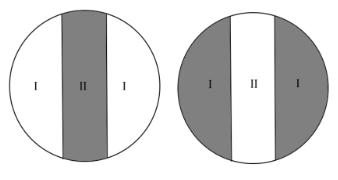
\includegraphics[width=0.4\textwidth]{../Images/Halbschatten.png}
    \caption{Looking through the polarimeter, there are
two fields visible, one at the edges and one
in the middle. Field I has a slightly dif-
ferent polarisation angle than field II. The
light from both fields passes through an ad-
justable polarisation filter, causing a differ-
ence of brightness.}
    \label{fig:halbschatten}
\end{figure}
\label{sec:optischeAktivitaet}
    \subsection{Theory}
    In many fields of study concentration analysis of unknown solutions is fundamental. To quickly determine the concentration of a solution, one can
    use the method of half-shadow polarimeter. This method is based on the fact that certain substances, such as sucrose, exhibit circular birefringence,
    which causes the plane of polarization of light to rotate as it passes through the solution. The angle of rotation is directly proportional to the
    concentration of the solution and the path length of the light through it. By measuring the angle of rotation, one can determine the concentration
    of the solution. \\
    For that method, the penumbral angle of the used polarimeter has to be determinded, by measuring the position of minimal brightness in field I and II
    and then subtracting the two angles from each other(see fig. \ref{fig:halbschatten}).

    \subsection{Measurements and results}
    The penumbral angle of the used polarimeter was determined to be $\psi = (11.60 \pm 0.73)^\circ$. \\
    Now the concentration of an unknown sucrose solution had to be determined. For that the 
    

